\begin{enumerate}[label=\thesubsection.\arabic*.,ref=\thesubsection.\theenumi]
\numberwithin{equation}{enumi}


\item The asymptotic Bode phase plot of 
%
\begin{align}
\label{eq:ee18btech11037_gs}
G(s) = \frac{k}{(s+0.1)(s+10)(s+{p_1})}
\end{align}
%
with k and $p_1$ both positive, is shown below.
\begin{figure}[!ht]
\centering
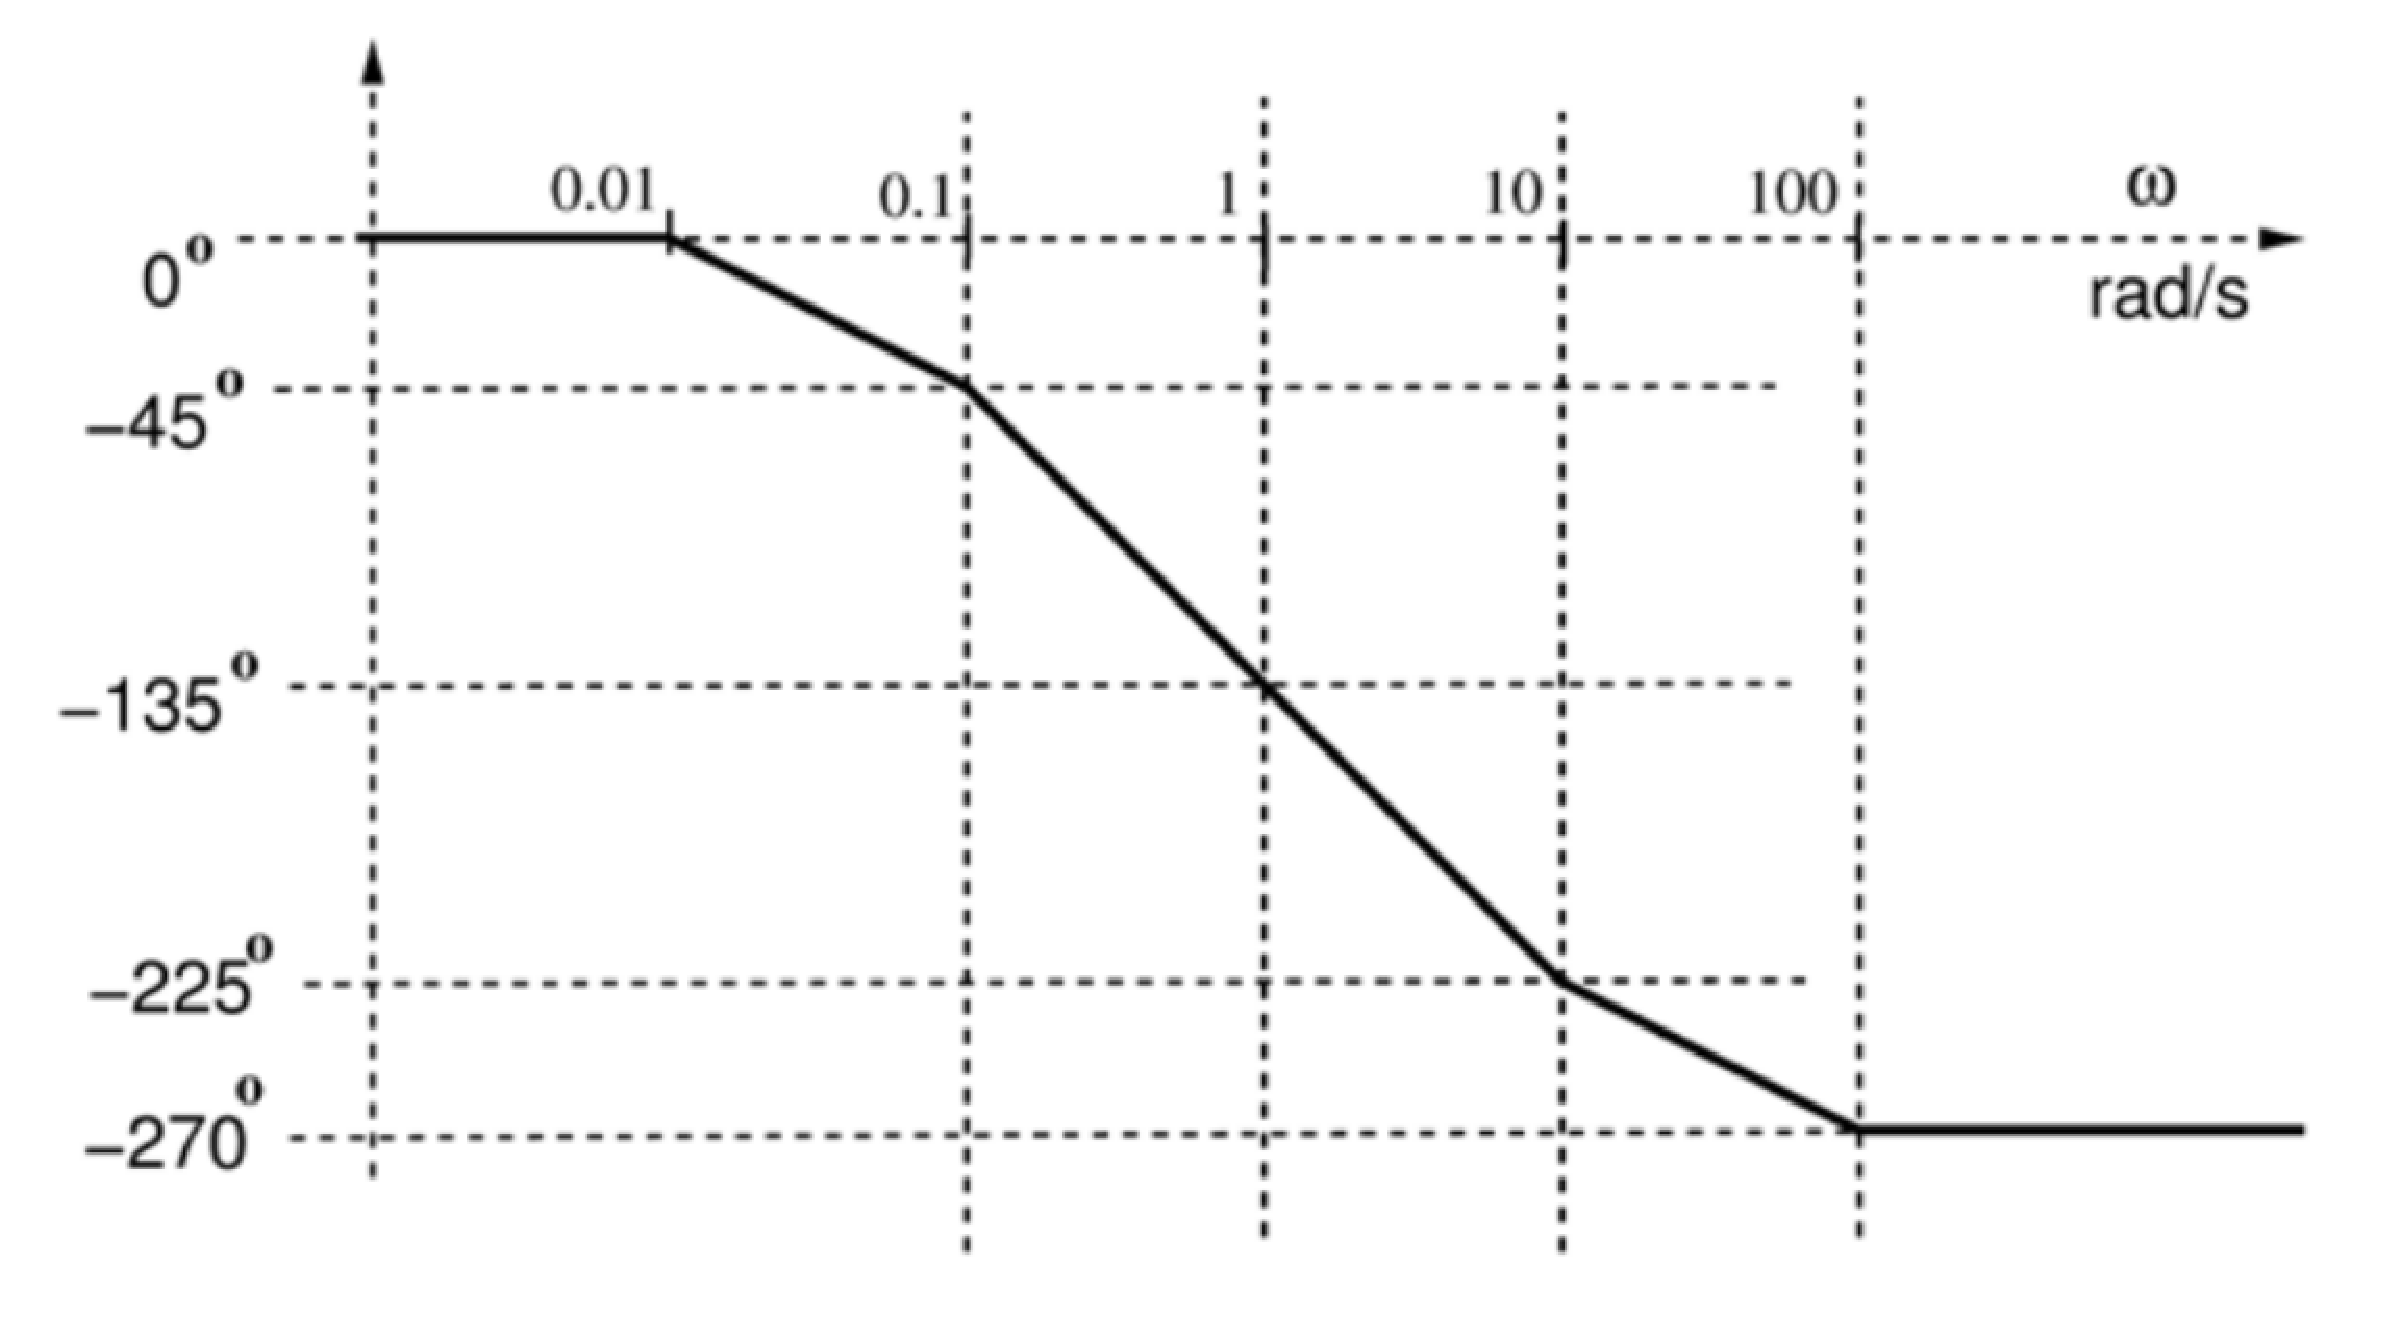
\includegraphics[width=\columnwidth]{figs/ee18btech11037/ee18btech11037.eps}
\caption{}
\label{fig:ee18btech11037}
\end{figure}
Find the value of \textit{$p_1$}.
\\
\solution
Bode phase plot for a transfer function having a single pole at p
\begin{align}
 \phi(\omega) = 
 \begin{cases} 
        0 & 0<\omega< \frac{p}{10} \\
      -45\times\brak{\log\brak{\frac{10\omega}{p}}}& \frac{p}{10}<\omega<10p \\
      -90 & 10p<\omega  
 \end{cases}
\end{align}

Phase plot of the transfer function \eqref{eq:ee18btech11037_gs},
\begin{align}
\label{eq:ee18btech11037_totalphase}
 \phi(\omega) = 
 \begin{cases} 
        0 & 0<\omega<0.01 \\
      -90-45\log(\omega)& 0.01<\omega<0.1 \\
      -135-90\log(\omega)& 0.1<\omega<10 \\
      -180-45\log(\omega)& 10<\omega<100 \\
      -90 & 100<\omega  
 \end{cases}
\end{align}
phase plot by considering only 0.1 and 10 poles is
\begin{align}
\label{eq:ee18btech11037_part_of_phase}
 \phi(\omega) = 
 \begin{cases} 
        0 & 0<\omega<0.01 \\
      -90-45\log(\omega)& 0.01<\omega<100 \\
      -180 & 100<\omega  
 \end{cases}
\end{align}
By comparing \ref{eq:ee18btech11037_totalphase} and \ref{eq:ee18btech11037_part_of_phase}, $\phi(\omega)$ remains
same till 0.1 so, 
\begin{align}
\frac{p_1}{10} = 0.1 \\
\implies p_1 = 1
\end{align}
the bode phase plots corresponding to the poles 0.1 and 10.
\begin{figure}[!ht]
\centering
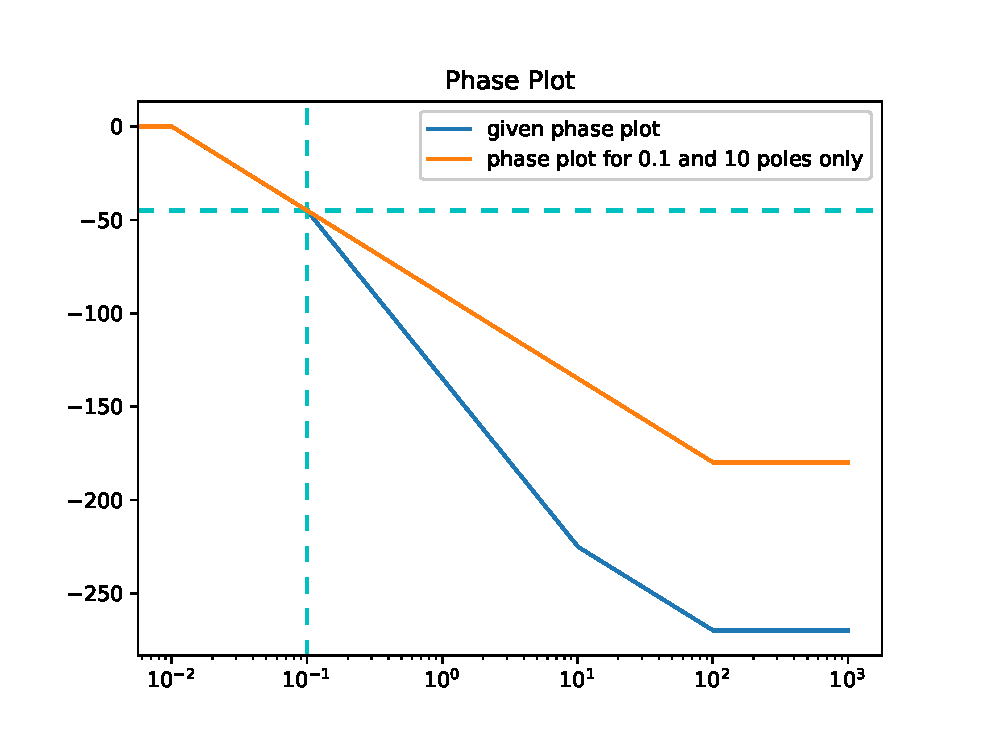
\includegraphics[width=\columnwidth]{figs/ee18btech11037/ee18btech11037_2.eps}
\caption{}
\label{fig:ee18btech11037_2}
\end{figure}

\item Find the value of $p_1$ using phase of the transfer function.
\\
\solution
\begin{align}
\phi(\omega) = -\tan^{-1} \brak{\frac{\omega}{0.1}}-\tan^{-1} \brak{\frac{\omega}{10}}-\tan^{-1} \brak{\frac{\omega}{p_1}}
\end{align}
From the plot,
\begin{align}
-45\degree = -\tan^{-1}\brak{\frac{0.1}{0.1}} -\tan^{-1}\brak{\frac{0.1}{10}} -\tan^{-1}\brak{\frac{0.1}{p_1}}
\end{align}
 $p_1$ is approximately 1, i.e, for $p_1$ in 0.95 to 1.05 the $\phi$ is approximately equals to $-45\degree$.
%
The following code plots Fig. \ref{fig:ee18btech11037_2}

\begin{lstlisting}
codes/ee18btech11037.py
\end{lstlisting}

\end{enumerate}
